% Qué tipo de documento estamos por comenzar:
\documentclass[a4paper]{article}
% Esto es para que el LaTeX sepa que el texto está en español:
\usepackage[spanish]{babel}
\selectlanguage{spanish}
% Esto es para poder escribir acentos directamente:
\usepackage[utf8]{inputenc}
\usepackage[T1]{fontenc}
\usepackage{bold-extra}
\usepackage{graphicx}
\usepackage{subfigure}
\usepackage{float}

%% Asigna un tamaño a la hoja y los márgenes
\usepackage[a4paper,top=3cm,bottom=2cm,left=3cm,right=3cm,marginparwidth=1.75cm]{geometry}

%% Paquetes de la AMS
\usepackage{amsmath, amsthm, amsfonts}
%% Para añadir archivos con extensión pdf, jpg, png or tif
\usepackage{graphicx}
\usepackage[colorinlistoftodos]{todonotes}
\usepackage[colorlinks=true, allcolors=blue]{hyperref}

\newcommand\tab[1][0.5cm]{\hspace*{#1}}

\title{Implementación de un Motor de Búsqueda de palabras en textos grandes}
\author{Daniel Palomino Paucar, Erick Tornero Tenorio, \\
Felipe Moreno Vera, Luis Colchado Soncco\\
  \small Universidad Católica San Pablo\\
  \small Arequipa,Perú
  \date{31 de agosto de 2018}
}

\begin{document}
\maketitle

 
\begin{abstract}
El área de estudios de estructura de datos tiene múltiples aplicaciones, ya sea desde almacenamiento de elementos multidimensionales, objetos, multimedia, etc. También tiene otras aplcaciones en organización de información (así como los hashes o listas) y preprocesado de información (como en bases de datos).

En el presente proyecto se llevó a cabo el desarrollo de una interfaz web que mediante una adecuada comunicación con un programa núcleo en C++ permite emular un search-engine similar a google, el cual busca palabras o cadenas de texto en un conjunto de documentos de textos provistos por Wikipedia, la búsqueda se realiza mediante una estructura de datos óptima, la cual se le conoce como Inverted Index.


\end{abstract}

%% Iniciamos "secciones" que servirán como subtítulos
%% Nota que hay otra manera de añadir acentos

\section{Descripción}

El presente trabajo muestra la manera de implementar un Motor de Búsqueda de palabras en textos grandes utilizando algoritmos de indexación y de consultas para mejorar el almacenado de texto y las consultas a dichos textos, ya sea palabras o frases. 

El proyecto consta de 3 partes fundamentales, donde en cada una se ha buscado la manera más óptima de implementación, para reducir el tiempo de consultas y búsqueda.

\section{Arquitectura del software}

La arquitectura del software se divide en 3 partes:
\begin{enumerate}
    \item Motor de Búsqueda.
    \item Consulta por consola.
    \item Servicio web.
\end{enumerate}

Tal como se muestra en la Figura \ref{figarchengine}:

\begin{figure}[H]
  \centering
  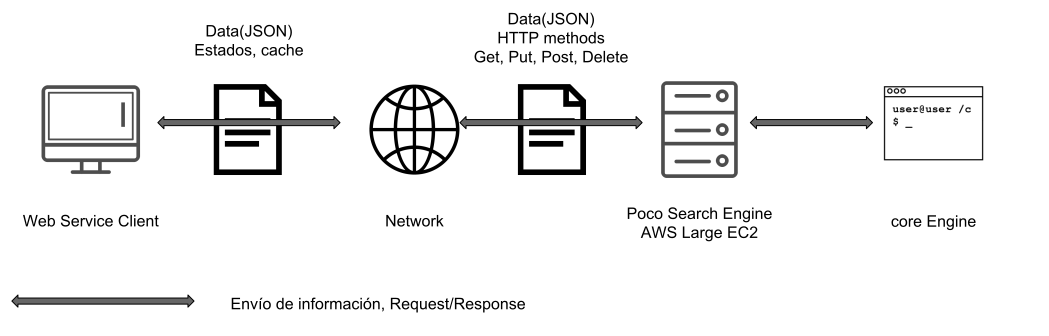
\includegraphics[width=16cm]{images/architecture.png}
  \caption{Arquitectura del search engine}
  \label{figarchengine}
\end{figure}

\subsection{Moto de Búsqueda}

El Core del Motor de Búsqueda esta basado en la estructura Inverted Index \cite{inverted_index}. 

Antes de usar dicha técnica de indexado, se pasó a hacer un preprocesado del texto transformando todo a minúsculas y agregando una similitud entre letras con tildes y sin tildes.

Una vez ya estandarizado los textos, se procede a indexar los tokens (palabras) de los textos en una estructura similar a una tabla hash, con la modificación que se contabilizan las frases/palabras en una tabla de frecuencias.

\subsubsection{Pre-procesamiento de texto}

Existen 3 etapas de procesamiento de texto:
\begin{enumerate}
    \item La primera etapa es la extracción de los documentos contenidos en los archivos, clasificándolos en la estructura $RetrievalData$ que permite diferenciar el identificar, el título y contenido de cada documento.
    \item La segunda parte es tokenizar el contenido de cada documento para eliminar los caracteres especiales (\textit{'@'}, \textit{'.'}, etc), y diferenciar las palabras que pueden contener información.
    \item La tercera etapa consiste en estandarizar todos los caracteres que serán introducidos al \textit{Inverted index} con el fin de minimizar el tiempo de consulta. Es decir considerar solo los caracteres que se les puede aplicar el \textit{LowerCase} o \textit{UpperCase}, esto es los caracteres del alfabeto. Además las vocales que llevan tíldes son cambiadas a su equivalente sin tilde.
    
\end{enumerate}


\subsubsection{Inverted-Index y Rankeo de Documentos} 

Dada la colección de documentos, asumimos que cada documento posee un identificador único al que hemos llamado $db\_index$. Durante la construcción del índex simplemente relacionamos cada documento con su identificador único.

La entrada de la indexación es una lista de tokens normalizada por cada documento, estructurada de tal forma que se relacione el token con el documento al que pertenece y la cantidad de ocurrencias que posee.

Cuando ocurre una búsqueda se extrae todas las relaciones encontradas de las palabras que componen la consulta y se ordena por orden de relevancia de acuerdo al siguiente criterio:

\begin{enumerate}
    \item Los documentos que tienen más repeticiones de todas las palabras tiene más relevancia.
    \item En caso de empate en el criterio anterior, se considera más relevante a aquellos documentos que posean más repeticiones de palabras individuales.
    \item En caso de no encontrar todas las palabras juntas en el mismo documento, se considera más relevante a los que contengan la mayor cantidad de palabras de la búsqueda en el mismo documento.
    \item En caso de empate en el criterio anterior, se considera más relevante a aquellos documentos que posean más repeticiones de palabras individuales.
\end{enumerate}

Es decir si se busca la frase $Comida\ Peruana$, primero aparecerán todos los documentos que contengan más repeticiones de todas las palabras $Comida$ y $Peruana$. Luego se mostrarán los documentos que contengan más repeticiones por palabra individual $Comida$ o $Peruana$\\

En otro caso de búsqueda $Guerra\ Curitiva$, por ejemplo, de no encontrarse ningún documento que contenga a ambas palabras juntas en un mismo documento, se mostrán los documentos que contengan más repeticiones por palabras individuales.\\

Finalemnte, si se buscara $Guerra Xsksjdh$, dado que la palabra $Xsksjdh$ no existe en ningún documento, se mostrarán como relevante a todos los documentos que sólo contengan la palabra $Guerra$ ordenados según la cantidad de ocurrencias en cada documento.

\subsection{Modo consulta por consola}

Se desarrolló una aplicación en entorno de consola, en este caso se tiene la opción de realizar la búsqueda por palabra, y ver el tiempo de la consulta en segundos y los resultados de 20 en 20, se puede también de poder ingresar al contenido de los resultados, seleccionando su indicador de contador en la pantalla. Además se tiene la opción de cancelar una búsqueda actual para poder realizar una nueva búsqueda de otra palabra.

\begin{figure}[H]
  \centering
  \includegraphics[width=14cm]{images/consola.png}
  \caption{Consulta por consola}
  \label{consola}
\end{figure}

\newpage

\subsection{Implementación de la conexión entre el programa Search-engine y el servicio web}

En esta sección se presenta la interconexión usando HTTP entre el Search-Engine desarrollado en C++ y la interface web hecha en js y html con un servicio en golang.

\subsubsection{Implementación de la interfaz web} 
Para la implementación de l ainterfaz web, se utilizo el webapp Sign, version 3.1, para el diseño de la interfaz.

\textbf{Templates}

Los templates, son ficheros con extension \textit{.tmpl} los cuales el lenguaje Golang interpreta y realiza un parse (se peude embeber información en dichos templates) dicha técnica es utilizada por todos ls framewprks web como dJango, ExpressJS, etc.

Los templates, permiten también manejar lenguaje de tipado html de forma nativa (sin cambiar la sintáxis) por lo cual hace más fácil la implementación y diseño de los componentes web.

\textbf{Golang}

Se utilizó el lenguaje de programación Golang para realizer el web service que se comunica con el servicio REST en cpp que se comunica con las consultas de la interfaz.

Se utilizó el protocolo HTTP por defecto, a diferencia de MQTT, HTTP se maneja de manera nativa en web services.

Además, la interfaz web se implementó utilizando el estilo applicaction min y fonts de google para el tipo de letra \ref{figsearchengine}.

\begin{figure}[H]
  \centering
  \includegraphics[width=8cm]{images/pocosearch.png}
  \caption{Vista principal del search engine}
  \label{figsearchengine}
\end{figure}

Al momento de realizar una consulta, nos retorna una lista de páginas de las cuales se identifican por Id de página (pero en la vista se presenta como título y contenido mínimo) y además el número de páginas en la parte inferior del documento de texto \ref{figresultsengine}.

\begin{figure}[H]
  \centering
  \includegraphics[width=8cm]{images/results.png}
  \caption{Resultados de una consulta en el search engine}
  \label{figresultsengine}
\end{figure}

\subsubsection{Web Server}

En lado del servidor se implemento un Web Server con el lenguaje de programación C++ y con la librería Boost. Esto nos permitió en especifico crear endpoints que con los métodos del protocolo HTTP logramos realizar la comunicación entre el core y el cliente en entorno Web. \\

\textbf{HTTP Protocol}

Los métodos HTTP tales como Get, Post, Delete y Update se utilizaron para realizar las consultas entre ambas partes del core search engine, el REST service y el web service.

Para la consulta desde clientes web usamos métodos GET, entre las consultas del web client y el core search engine usamos métodos post.



\section{Resultados}

Se obtuvieron los siguientes resultados en promedio:

\begin{enumerate}
    \item Tiempo de indexación: 168 segundos
    \item Cantidad de Documentos Indexados: 259599
    \item Memoria utilizada: 2.8 GB
    \item Tiempo promedio de consulta: 2.3 ms
\end{enumerate}

Se hicieron pruebas también con 11, 22, 33, 44 y 57 files utilizando, las palabras serie1: "maestria", serie 2:"maestria en ciencias" y serie3: "maestria en ciencias de la computacion". Los resultados fueron los siguientes:

\begin{figure}[H]
  \centering
  \includegraphics[width=8cm]{images/grafica.jpeg}
  \caption{Resultados}
  \label{grafica}
\end{figure}


\section{Limitaciones}

A pesar de los buenos resultados en cuestión de tiempo de indexación y búsqueda de frases y/o palabras, el presente trabajo posee limitaciones en cuanto a recomendaciones de otras palabras relacionadas cuando la palabra o frase original no se encuentra en ningún documento indexado.

Otra limitación a tomar en cuenta es el alto consumo de memoria para la indexación.

\section{Trabajos futuros}

El presente proyecto implementado podría incrementar su funcionalidad realizando búsquedas a páginas web para lo cual se tendría que implementar diferentes técnicas de conexión a la world wide web y extraer información, así como realizar nuevos parsers de estandarización de los miles de textos contenidos ahí. Y a su vez, se podría incrementar su eficiencia y rápidez (la cual se necesitará conforme vaya aumentando el número de información de textos que se tenga) para que las consultas se mantengan o disminuyan el tiempo de respuesta.

\section{Conclusiones}

Podemos mencionar la siguientes conclusiones importantes:

\begin{itemize}

    \item El Inverted Index es una estructura óptima para la creación de motores de búsqueda de palabras en textos grandes debido a su fácil implementación y adecuado performance en tiempo de búsqueda.
    
    \item Siendo el consumo de memoria un factor crítico en la aplicación, el Hardware necesario para la puesta en producción debe poseer un adecuado dimensionamiento.
    
    \item El haber integrado la estructura de indexación (Inverted Index) al core del webserver permite la creación de una aplicación multi-usuario.
    
    
\end{itemize}


\section{Distribución del trabajo}

Para el desarrollo del presente proyecto, las tareas fueron divididas entre todos los colaboradores de la siguiente manera:
\begin{itemize}
    \item \textbf{Desarrollo del Inverted Index} El desarrollo de la estructura Inverted Index, estructura la cual clasifica y asigna una determinada key a las palabras o cadenas de strings, así como también el desarrollo del cliente de consola (CLI) para realizar las búsquedas de palabras en los textos estuvo a cargo de Daniel Palomino. 
    
    \item \textbf{Desarrollo del Parser} El desarrollo de la estandarización de información (textos) de tal forma que sea más fácil acceder y leer, estuvo a cargo de Erick Tornero.
    
     \item \textbf{Conexión web service - programa}
     
     La implementación, configuración del Web Server en C++ con Boost library, el cual permite el intercambio de información por medio del protocolo HTTP, además de la configuración del servicio Web en el lenguaje Go y su configuración en la instancia EC2 en AWS, estuvo a cargo de Luis Colchado.
    
    \item \textbf{Interfaz Web}
    
    El diseño y organización de los componentes visuales de la interfaz web, así como el desarrollo del web service de la interfaz web y la adaptación de templates en Golang y además de la funcionalidad de responsive en páginas web estuvo a cargo de Felipe Moreno.
\end{itemize}

\section{Link repositorio Github}

El link del repositorio es \url{https://github.com/AED-MINIGOOGLE/minigoogle}.

\section{Link Video}

El link del video es \url{https://youtu.be/7ZhRS3Xr06o}

\section{Link de la simulación web del Search Engine}

El link de la página web que emula el search engine es \url{http://minigoogle.gescloud.io}

\begin{thebibliography}{9}

\bibitem{inverted_index}
NLP Stanford, \url{https://nlp.stanford.edu/IR-book/html/htmledition/a-first-take-at-building-an-inverted-index-1.html}. Last visited 30/08/2018.

\bibitem{video}
Erik Demaine. Session 16: Strings [Archivo de video]. Recuperado de https://ocw.mit.edu/courses/electrical-engineering-and-computer-science/6-851-advanced-data-structures-spring-2012/lecture-videos/session-16-strings/
\end{thebibliography}

\end{document}